%----------------------------------------------------------------------------------------
%	Metropolia Thesis LaTeX Template
%----------------------------------------------------------------------------------------
% License:
% This work is licensed under the Creative Commons Attribution 4.0 International License.
% To view a copy of this license, visit http://creativecommons.org/licenses/by/4.0/.
%
% However, this license apply to this template. As a template, it is supposed to be
% modified for your own needs (with your thesis content). For this reason, if you use
% this project as a template and not specifically distribute it as part of a another
% package/program, we grant the extra permission to freely copy and modify these files as
% you see fit and even to delete this copyright notice.
% In short, you are free to publish your thesis under whatever license you wish, even
% keep the all rights reserved to you.
%
% Authors:
% Panu Leppäniemi, Patrik Luoto, Mikaa Oni and Patrick Ausderau
%
% Credits:
% Panu Leppäniemi: abstract, def, cleaning,...
% Patrik Luoto: title page, abstract in Finnish, abbreviation, math,...
% Mikaa Oni: switch to biber biblatex
% Patrick Ausderau: initial version, style, table of content, bibliography, figure,
%                   appendix, table, source code listing,...
%
% Please:
% If you find mistakes, improve this template and alike, please contribute by sharing
% your improvements and/or send us your feedback there:
% https://github.com/panunu/metropolia-thesis-latex
% And of course, if you improve it, add yourself as an author.
%
% Compiler:
% Use XeLaTeX as a compiler. LuaLaTeX works too.
% Typical compilation:
% # minted require -shell-escape to run  external script.
% # -8bit avoid ^^I for tabs in minted.
% $ xelatex -shell-escape -8bit main
% # If any change in the bibliography
% $ biber main
% # If any change with the abbreviation or acronym
% $ makeglossaries main
% #Then compile again
% $ xelatex -shell-escape -8bit main
% #And if still some citation or label warnings, compile once more
% $ xelatex -shell-escape -8bit main

%----------------------------------------------------------------------------------------
%	THESIS INFO
%----------------------------------------------------------------------------------------

% All general information (main language, title, author (you), degree programme, major
% option, etc.)
% Edit the file chapters/0info.tex to change these information
% !TEX root = ../main.tex

\documentclass[12pt,a4paper,oneside,article]{memoir}%Do not touch this first line ;)

% Global information (title of your thesis, your name, degree programme, major, etc.)

\def\bilingual{yes}%For Finnish students, you must have 2 abstracts, one in English and one in your native language (Finnish or Swedish), so "yes", your thesis is bilingual.
%\def\bilingual{no}%For international student writing in English, only one language and one abstract.

\def\thesislang{finnish} %change this depending on the main language of the thesis.
%\def\thesislang{english} % "english" is the only other supported language currently. If someone has the swedish, please contribute!

\def\secondlang{english} %if the main language is Finnish (or Swedish), you must have 2 abstracts (one in Finnish (or Swedish) and one in English)
%\def\secondlang{finnish}
%If the main language is English and that you are native Finnish (or Swedish) speaker, you must have also abstract in your native language on top of the English one.

\author{Nimi/Name} %your first name and last name

%\def\alaotsikko{Alaotsikko/Subtitle} %DISABLED, seems not to be an option with the 2018 template. If you really need it, uncomment and modify style/title.tex accordingly.

%License
%When publishing your thesis to theseus.fi, you can keep all rights reserved to you,
%or use one of the Creative Commons https://creativecommons.org/licenses/?lang=en
%This attribute will set the license in the metadata of the generated pdf.
%possible options (case sensitive):
%all (keep all rights reserved to yourself)
%by (Attribution)
%by-sa (Attribution-ShareAlike)
%by-nd (Attribution-NoDerivs)
%by-nc (Attribution-NonCommercial)
%by-nc-sa (Attribution-NonCommercial-ShareAlike)
%by-nc-nd (Attribution-NonCommercial-NoDerivs)
%Note that theseus do not accept dedication to public domain CC0
\def\thesiscopy{all}

%Finnish section, for title/abstract
\def\otsikko{Opinnäytetyön otsikko}
\def\tutkinto{Tutkinto (esim. Insinööri (AMK))} % change to your needs, e.g. "YAMK", etc.
\def\kohjelma{Koulutusohjelma (esim. Tieto\textendash ja viestintätekniikka)}
\def\suuntautumis{Ammatillinen pääaine (esim. Mobile Solutions)}
\def\thesisfi{Insinöörityö}%was Opinnäytetyö
\def\ohjaajat{
Titteli Etunimi Sukunimi\newline
Titteli Etunimi Sukunimi
}
\def\tiivistelma{
Tämä on tiivistelmän ensimmäinen kappale. Tiivistelmän kappaleet loppuvat komentoon newline, jotta saadaan yksi tyhjä rivi aikaiseksi. \newline

Tämä on tiivistlemän toinen kappale.
}
\def\avainsanat{avainsana, avainsana}
\def\aihe{Lyhyt kuvaus opinnäytetyöstä. Max 255 merkkiä.}%for the pdf metadata/properties. If not used, empty it and also the \def\subject.

%English section, for title/abstract
\title{Your title here}
\def\metropoliadegree{Bachelor of Engineering} % change to your needs, e.g. "master", etc.
\def\metropoliadegreeprogramme{your degree programme (e.g. Information Technology)}
\def\metropoliaspecialisation{your major option (e.g. Mobile Solutions)}
\def\thesisen{Bachelor’s Thesis} % change to your need, e.g. master's
\def\metropoliainstructors{
First name Last name, Title (e.g.: Project Manager)\newline
First name Last name, Title (e.g.: Principal Lecturer)
}
\def\abstract{
Abstract content. To force newline between paragraph in the abstract, you must have both a empty line and the newline command. \newline

beginning of second paragraph\ldots
}
\def\metropoliakeywords{keyword, keyword}
\def\subject{short description of the thesis. Max 255 characters.}%for the pdf metadata/properties. If not used, empty it and also the \def\aihe.


%----------------------------------------------------------------------------------------
%	GLOBAL STYLES
%----------------------------------------------------------------------------------------

% If you need extra package, etc. modify the style/style.tex file.
% If you are using Windows OS, you will need to change default font to Arial in that
% style/style.tex file (or install Liberation Sans font to your system).
% If you are using MacOS or linux, make sure you have Liberation Sans font installed.
% Global style. Normally should not be edited.
% If you use windows OS, eventually change \setmainfont to Arial
% Check around commit https://github.com/panunu/metropolia-thesis-latex/commit/a0c15ac77bab1a52c59c517a18080938e57bf5ef
% to see how the font files were manually added (after downloading them: https://pagure.io/liberation-fonts/ )

%\usepackage[l2tabu, orthodox]{nag}%check for obsolete packages (with outdated nag package?)

%condition e.g. for adding or not space in TOC,...
\usepackage{etoolbox}
\ifdefstring{\bilingual}{yes}{
  \usepackage[\secondlang,\thesislang]{babel}% finnish (or swedish) and english
}{
  \usepackage[\thesislang]{babel}% english only
}
\usepackage{iflang}
\usepackage{amsmath}
\usepackage{amsfonts}%extra mathematical symbols
\usepackage{amssymb}
\usepackage{fontspec}
\usepackage{titlesec}
\usepackage{mathtools}%enhance the appearance of documents containing a lot of mathematics
\usepackage[amssymb]{SIunits}
\usepackage[version=3]{mhchem}
\usepackage{tikz} % mindmaps, flowcharts, piecharts, examples at http://www.texample.net/tikz/examples/
\usetikzlibrary{shapes.geometric, arrows}

\usepackage{ragged2e}
\IfLanguageName{finnish}{
  \RaggedRight%2021 template, align left and hyphennization for Finnish version
  \setlength{\RaggedRightRightskip}{0pt plus 1fil}%TODO: fix the Overfull/Underfull warnings when \RaggedRight (likely in title and abstact)
}{}
\makeatletter
  \let\@gnewline\@raggedtwoe@saved@gnewline% Restore original functionality of \newline
  \let\\\@raggedtwoe@savedcr% Restore original functionality of \\
\makeatother

%for compact list
\usepackage{enumitem}
%\usepackage{verbatim}%for block comment
%forcing single line spacing in bibliography
\DisemulatePackage{setspace}
\usepackage{setspace}
%\usepackage{eurosym}%euro symbol
%try to count
\usepackage{totcount}
%insert source code
%require -8bit -shell-escape in the xelatex compile command
%if compiling locally, consider options cachedir=minted,outputdir=~/.tex
\usepackage[newfloat]{minted}
\setminted{tabsize=2,linenos,breaklines,breaksymbolleft={\quad},baselinestretch=1}
\setmintedinline{breaklines,breakanywhere}
\usepackage[singlelinecheck=false]{caption}
%force the width of a table instead of column
\usepackage{tabularx}
\usepackage{booktabs} %why not booktabs? :3

\usepackage{csquotes}% avoid warning with babel

\usepackage{float} % For forced figure location with modifier H (\begin{figure}[H])
\usepackage{wrapfig}

% citep-macro for reference with period inside square brackets [1.]
\newcommand{\citep}[1]{
 \renewcommand\citeright{.]}
 \cite{#1}
 \renewcommand\citeright{]}
}

%set date format to D.M.YYYY
\def\pvm{\the\day.\the\month.\the\year}
%set date format to D Month YYYY
\usepackage[en,useregional=false]{datetime2}
\DTMsetup{datesep=.}
\DTMnewdatestyle{dMonthyyyy}
{%
  \renewcommand{\DTMdisplaydate}[4]{%
    \number##3 % day
    ~% separator
    \DTMenglishmonthname{##2}% month name
    ~% separator
    \number##1% year
  }%
  \renewcommand{\DTMDisplaydate}[4]{%
    \DTMdisplaydate{##4}{##3}{##2}{##1}%
  }%
}
\DTMsetdatestyle{dMonthyyyy}
\date{\today}

\newcommand\tn[1]{\textnormal{#1}} %use \tn instead of \textnormal
\newcommand\reaction[1]{\begin{equation}\ce{#1}\end{equation}} %\reaction{} for chemical reactions

%NORMAL TEXT
%all text, title, etc. in the same font: Arial
%NOTE: fontname is case-sensitive
\setmainfont[Scale=0.98]{Liberation Sans}
%line space
\linespread{1.46}
\AtBeginEnvironment{tabular}{\singlespacing}
%\doublespacing
%margin
%geometry moved after hyperref
\setlength{\parindent}{0pt} %first line of paragraph not indented
\setlength{\parskip}{16.5pt} %one empty line to separate paragraph
%list with small line space separation
\tightlists
\setlist[itemize]{before=\singlespacing,itemsep=6pt,leftmargin=63pt,labelsep=22pt,topsep=1.5pt,partopsep=0pt,after=\vspace{-22pt}\newline}
\setlist[enumerate]{before=\singlespacing,itemsep=6pt,leftmargin=63pt,labelsep=22pt,topsep=1.5pt,partopsep=0pt,after=\vspace{-22pt}\newline}

%IMAGE - FIGURE
%the figures should be placed in the "illustration" folder
\graphicspath{{illustration/}}
%figure number without chapter (1.1, 1.2, 2.1) to (1, 2, 3)
\counterwithout{figure}{chapter}
%border around images
\setlength\fboxsep{0pt}
\setlength\fboxrule{0.5pt}
%space after figure caption (and other float elements)
\setlength{\belowcaptionskip}{-7pt}
\setlength{\intextsep}{16.5pt}%space around floats
\AtBeginEnvironment{table}{\addvspace{16.5pt}}

%TABLE
\counterwithout{table}{chapter}

%SOURCE CODE
\newenvironment{code}{\captionsetup{type=listing}}{}
\IfLanguageName{finnish}{\SetupFloatingEnvironment{listing}{name=Koodiesimerkki}}{}%was Listaus
%\counterwithout{lstlisting}{chapter}
%moved after begin document, otherwise does not compile

%TOC
%change toc title
\IfLanguageName{finnish}{\addto{\captionsfinnish}{\renewcommand*{\contentsname}{Sisällys}}}{}
%remove dots
\renewcommand*{\cftdotsep}{\cftnodots}
%chapter title and page number not in bold
\renewcommand{\cftchapterfont}{\normalfont}
\renewcommand{\cftchapterpagefont}{\normalfont}
%sub section in toc
\setcounter{tocdepth}{2}
%subsection numbered
\setcounter{secnumdepth}{2}
\renewcommand{\tocheadstart}{\vspace*{-33.5pt}}
\renewcommand{\printtoctitle}[1]{\fontsize{13.5pt}{13.5pt}\bfseries #1\vspace*{-4pt}}
%\renewcommand{\aftertoctitle}{\vspace*{-22pt}\afterchaptertitle}
%spacing after a chapter in toc
\preto\section{%
  \ifnum\value{section}=0\addtocontents{toc}{\vskip11pt}\fi
}
%spacing after a section in toc
\renewcommand{\cftsectionaftersnumb}{\vspace*{-3pt}}
%spacing after a subsection in toc
\renewcommand{\cftsubsectionaftersnumb}{\vspace*{-1pt}}
%appendix in toc with "Appendix " + num
\IfLanguageName{finnish}{
  \renewcommand*{\cftappendixname}{Liite\space}
  \renewcommand{\appendixtocname}{Liitteet}
}{\renewcommand*{\cftappendixname}{Appendix\space}}
%appendix header
\IfLanguageName{finnish}{\def\appname{Liite\space}}{\def\appname{Appendix\space}}

%TITLES
%chapter title
%\clearforchapter{\clearpage}
\titleformat{\chapter}
{\fontsize{14pt}{14pt}\bfseries\linespread{1}}%\clearpage
{\thechapter}{.5cm}{}
\titlespacing*{\chapter}{0pt}{-.42cm}{.5pt}
\titleformat{\section}
{\fontsize{13.5pt}{13.5pt}\normalfont}
{\thesection}{.5cm}{}
\titlespacing*{\section}{0pt}{9pt}{0pt}
\titleformat{\subsection}
{\fontsize{12.7pt}{12.7pt}\normalfont}
{\thesubsection}{.5cm}{}
\titlespacing*{\subsection}{0pt}{11pt}{0pt}


%QUOTE
\renewenvironment{quote}
{\list{}{\rightmargin=0pt\leftmargin=2.2cm\topsep=-14pt}%
  \item\relax\singlespacing}%\fontsize{10pt}{10pt}
    {\vspace{8pt}\endlist}

%BIBLIOGRAPHY
%TODO: toggle for Harward v.s. Vancouver
\usepackage[
backend=biber,
bibencoding=utf8,%
citetracker=true,%
isbn=false,%
doi=false,%
url=true,%
usetranslator=true,%
bibstyle=ext-authoryear,%
citestyle=numeric-comp,%
sorting=none,%
sortcites=true,%
block=none,%
terseinits=false,%
giveninits=false,%
maxbibnames=99,%
]{biblatex}

\setlength{\bibitemsep}{11pt}
\setlength{\biblabelsep}{1cm}%with 1cm horizontal gap

\makeatletter
\RequireBibliographyStyle{numeric}
\makeatother

% set right format
\renewcommand*{\multicitedelim}{;\space}
\renewcommand*{\multinamedelim}{;\space}
\renewcommand*{\finalnamedelim}{~\&\space}
\DeclareFieldFormat{biblabeldate}{#1}
\DeclareDelimFormat[bib]{nameyeardelim}{\addperiod\space}
%\DeclareNameAlias{sortname}{last-first} % deprecated
\DeclareNameAlias{default}{family-given}
\DeclareFieldFormat{labelnumberwidth}{#1} % remove () from label number
\DeclareFieldFormat{title}{#1} % normal font for title
\DeclareFieldFormat{citetitle}{#1}
\DeclareFieldFormat{journaltitle}{#1} % remove underline
\DeclareFieldFormat*{url}{%
\ifentrytype{online}{\IfLanguageName{finnish}{Verkkoaineisto}{Online}\addperiod\space}{}%
\ifentrytype{video}{Video\addperiod\space}{}%
\textless\url{#1}\textgreater\addperiod
} % you can modify how to url looks here
%TODO: remove leading 0 for day and month for Finnish dates
\DeclareFieldFormat{urldate}{\space\bibstring{urlseen}\space#1} % remove () from date
%try set translation to biblio
\DefineBibliographyStrings{english}{%
    urlfrom = {available at},%
    urlseen = {Visited on},%
    fromenglish = {from English},%
    fromfinnish = {from Finnish},%
    fromgerman = {from German},%
    fromjapanese = {from Japanese},%
}
\DefineBibliographyStrings{finnish}{%
  %  urlfrom={Linkki: },%
    urlfrom = {},%
    urlseen = {Luettu},%
    fromjapanese = {japanista},%
    fromenglish = {englannista},%
    fromfinnish = {suomesta},%
    fromgerman = {saksasta},%
}
{
  %new cite command: "Vancouver Short"
  \DeclareCiteCommand{\citeVS}
    {\usebibmacro{prenote}}
    {\usebibmacro{author}, \usebibmacro{title}}
    {\multicitedelim}
    {\usebibmacro{postnote}}

  % new cite command: "Vancouver Short Collection" - necessary when referencing whole collections.
  \DeclareCiteCommand{\citeVSc}
    {\usebibmacro{prenote}}
    {\usebibmacro{editor}, \usebibmacro{title}}
    {\multicitedelim}
    {\usebibmacro{postnote}}
}

% when citing multiple sentences/entire paragraph, add a dot inside the brackets
\DeclareCiteCommand{\citep}[\mkbibbrackets]
  {\usebibmacro{cite:init}%
    \usebibmacro{prenote}}
  {\usebibmacro{citeindex}%
     \usebibmacro{cite:comp}}
  {\multicitedelim}
  {\usebibmacro{postnote}\addperiod}

\addbibresource{biblio.bib}% for biblatex you need out \printbibliography too

%count the appendices (since the chapter counter is reset after \appendix).
%! require to complie 2 times
\regtotcounter{chapter}

% metadata (title, author, lang,...) for accessibility, etc.
\usepackage{hyperref}
\usepackage{hyperxmp}
\def\isolang{\IfLanguageName{finnish}{fi}{en}} %iso code (based on main language)
\ifdefstring{\thesiscopy}{all}{%
    \def\copyen{Copyright \textcopyright\ \the\year{}, \theauthor}
    \def\copyfi{Kaikki oikeudet pidätetään.  \textcopyright\ \the\year{}, \theauthor}
  }{%
    \usepackage[type={CC},modifier={\thesiscopy},version={4.0},]{doclicense}
    \def\copyen{\thetitle\ \textcopyright\ \the\year{} by \theauthor\ is licensed under \doclicenseLongNameRef}
    \def\copyfi{\otsikko\ \textcopyright\ \the\year{}, jonka tekijä on \theauthor, on lisensoitu \doclicenseLongNameRef}
}
\hypersetup{%
  pdfdisplaydoctitle,
  %breaklinks=true,%searching for overfull warnings
  pdfencoding=auto,
  bookmarksdepth=subsection,
  unicode=true,
  keeppdfinfo=true,
  pdflang={\isolang},
  pdfmetalang={\isolang},
  pdftitle={\IfLanguageName{finnish}{\otsikko}{\thetitle}},
  pdfkeywords={\IfLanguageName{finnish}{\avainsanat}{\metropoliakeywords}},
  pdfcopyright={\IfLanguageName{finnish}{\copyfi}{\copyen}},
  pdfsubject={\IfLanguageName{finnish}{\aihe}{\subject}},
}

\ifdefstring{\bilingual}{yes}{%metadata (title and copyright) in multiple language
  \XMPLangAlt{\IfLanguageName{finnish}{en}{fi}}{%
    pdftitle={\IfLanguageName{finnish}{\thetitle}{\otsikko}},
    pdfcopyright={\IfLanguageName{finnish}{\copyen}{\copyfi}},
    pdfsubject={\IfLanguageName{finnish}{\subject}{\aihe}},
  }
}{}
\urlstyle{same}

%moved after hyperred as can cause conflicts
\usepackage{pdfcomment}%try the alt text for graphics
\usepackage{accsupp}
\newcommand{\AltText}[2]{\BeginAccSupp{method=pdfstringdef,unicode,Alt={{#1}}}\pdftooltip{{#2}}{{#1}}\EndAccSupp{}}

\usepackage[top=2.5cm, bottom=3cm, left=4cm, right=2cm, nofoot]{geometry}

\usepackage{pgfplots} %simple plots etc
\pgfplotsset{compat=1.16}
\usepackage{pgfplotstable}

% Abbreviations, acronym and glossary, in case of bug, remove temporary the noredefwarn
\usepackage[acronym,toc,nonumberlist,section=chapter,noredefwarn]{glossaries}%xindy,%toc, ,nomain
\newglossarystyle{mystyle}{%
  \setglossarystyle{list}% base this style on the list style
  \renewcommand*{\glossentry}[2]{%
  \item[\glsentryitem{##1}%
    \glstarget{##1}{\glossentryname{##1}:}]
  \glossentrydesc{##1}\glspostdescription\space ##2}
}
\setglossarystyle{mystyle}

\renewcommand*{\glsclearpage}{}

% Normally, you do not need to modify the title style. It's content comes from the
% chapters/0info.tex file.
% TITLE PAGE
% Normally, you should not edit this file.

\makeatletter
\renewcommand{\maketitle}{
\newgeometry{left=4cm,top=2.7cm}
\thispagestyle{empty}

\AltText{\IfLanguageName{finnish}{Metropolia Ammattikorkeakoulu.}{Metropolia University of Applied Sciences.}}{
\includegraphics[width=9.1cm,keepaspectratio]{Metropolia_L_oranssi}}

\IfLanguageName{finnish}{
\vspace*{1.36cm}
}{
\vspace*{1.18cm}
}
\tn{\large\theauthor\\[9.2mm]{\fontsize{27.5pt}{27.5pt}\normalfont\color[RGB]{155,50,35}\IfLanguageName{finnish}{\otsikko}{\thetitle}}}%\\[22pt]\LARGE\alaotsikko\\[1.75cm]}

\vspace*{2.38cm}
{\setstretch{1.512}
\IfLanguageName{finnish}{
  Metropolia Ammattikorkeakoulu\\
  \tutkinto \\
  \kohjelma \\
  \thesisfi\\
  \pvm % D.M.YYYY date format for Finnish.
} {
  Metropolia University of Applied Sciences\\
  \metropoliadegree \\
  \metropoliadegreeprogramme \\
  \thesisen\\
  \@date %D Month YYYY for English
}
}
\clearpage
\restoregeometry
}
\makeatother



%----------------------------------------------------------------------------------------
%	ABBREVIATION AND GLOSSARY
%----------------------------------------------------------------------------------------

% Add/edit all your acronyms, abbreviations, glossary entries, etc. definitions in
% chapters/0abbr.tex file.
% You can have as many as you wish. Only the ones you use in your text (inserted with
% \gls{} command) will print in the Glossary/Lyhenteet.
% Generate the glossary
\makeglossaries

% Acronyms, abbreviations, etc.

\newacronym{html}{HTML}{HyperText Markup Language}
\newacronym{sql}{SQL}{Structured Query Language}
\newacronym{io}{I/O}{Input/Output}
\newacronym{ram}{RAM}{Random Access Memory}
\newacronym{php}{PHP}{Hypertext Preprocessor}
\newacronym{wysiwym}{WYSIWYM}{What You See Is What You Mean}
\newacronym{isbn}{ISBN}{International Standard Book Number}
\newacronym{url}{URL}{Uniform Resource Locator}
\newacronym{doi}{DOI}{Digital Object Identifier}

% Glossary entries

\newglossaryentry{part_key}{
	name={partition key},
	description={a column or set of columns from the same table whose consolidated value decide the partition for a given data}
}
\newglossaryentry{thesis}{
	name=thesis,
	description={a written essay one submitted for a university degree},
	plural=theses
}
\newglossaryentry{latex}
{
	name=\LaTeX{},
	description={Is a mark up language specially suited for scientific documents}
}

\newglossaryentry{maths}
{
	name=mathematics,
	description={Mathematics is what mathematicians do}
}




%----------------------------------------------------------------------------------------
%	DOCUMENT STARTS HERE...
%----------------------------------------------------------------------------------------

\begin{document}
\IfLanguageName{finnish}{
}{
  \raggedright%2021 template, align left, no hyphennization for English version
}
\counterwithout{listing}{chapter}

%----------------------------------------------------------------------------------------
%	TITLE PAGE
%----------------------------------------------------------------------------------------

% Title header. You should not edit that file.

%page number always on the top right, clear the "chapter/section" head
\pagestyle{myheadings}
\markright{}
%clear chapter "title" foot page
\makeevenfoot{plain}{}{}{}
\makeoddfoot{plain}{}{}{}



\maketitle
\newpage

%----------------------------------------------------------------------------------------
%	ABSTRACT / Tiivistelmä
%----------------------------------------------------------------------------------------

% If you are international student writing in English, ignore the Finnish abstract.
% If you are Finnish citizen, you must have 2 abstracts, one in Finnish (or Swedish
% depending on your mother tongue) and one in English regardless of the main language of
% your thesis. Normally, you do not need to modify the abstract style. It's content comes
% from the chapters/0info.tex file.
\ifdefstring{\bilingual}{no}{%
    % Abstract in English
% Normally, you should not edit this file. Everything comes from chapter/0info.tex

\pagestyle{empty} %remove page number
\newgeometry{top=2.45cm,left=4cm,right=.5cm}
\begin{otherlanguage}{english}
{\large\textbf{Abstract}}
{\renewcommand{\arraystretch}{1.1}
  \begin{tabular}{@{}p{4.7cm} >{\raggedright\arraybackslash}p{10.8cm}@{}}
  Author: & \makeatletter\@author\makeatother
  \\
  Title: & \makeatletter\@title\makeatother
  \\
  Number of Pages: & \pageref*{LastPage} pages + \total{chapter} appendices
  \\
  Date: & \makeatletter\thedate\makeatother
  \\[6.5mm]
  Degree: & \metropoliadegree
  \\
  Degree Programme: & \metropoliadegreeprogramme
  \\
  Professional Major: & \metropoliaspecialisation
  \\
  Supervisors: & \metropoliainstructors
  \\[6mm]
  \cmidrule[.7pt](l{-.15em}r{5.5em}){1-2}
  \\
  \multicolumn{2}{>{\raggedright}p{15.5cm}}{
    \abstract
  }
  \\
  \\
  Keywords: & \metropoliakeywords
  \\
\end{tabular}
}
\end{otherlanguage}
\restoregeometry
\clearpage


    }{%
    \IfLanguageName{finnish}{%order of abstracts based on main language and spacing hell
        % Abstract in Finnish
% Normally, you should not edit this file. Everything comes from chapter/0info.tex

\pagestyle{empty} %remove page number
\newgeometry{top=1.5cm,left=4cm,right=.5cm}
\begin{otherlanguage}{finnish}
{\large\textbf{Tiivistelmä}}
{\renewcommand{\arraystretch}{1.1}
  \begin{tabular}{@{}p{4.7cm} >{\raggedright\arraybackslash}p{10.8cm}@{}}
  Tekijä: & \makeatletter\@author\makeatother
  \\
  Otsikko: & \otsikko
  \\
  Sivumäärä: & \pageref*{LastPage} sivua + \total{chapter} liitettä
  \\
  Aika: & \pvm
  \\[6.5mm]
  Tutkinto: & \tutkinto
  \\
  Tutkinto-ohjelma: & \kohjelma
  \\
  Ammatillinen pääaine: & \suuntautumis
  \\
  Ohjaajat: & \ohjaajat
  \\[11mm]
  \cmidrule[.7pt](l{-.15em}r{5.5em}){1-2}
  \multicolumn{2}{>{\raggedright}p{15.5cm}}{
  \vspace{.2mm}
  \tiivistelma
  }
  \\
  \\
  Avainsanat: & \avainsanat
  \\
\end{tabular}
}
\end{otherlanguage}
\restoregeometry
\clearpage


        % Abstract in English
% Normally, you should not edit this file. Everything comes from chapter/0info.tex

\pagestyle{empty} %remove page number
\newgeometry{top=1.77cm,left=4cm,right=.5cm}
\begin{otherlanguage}{english}
{\large\textbf{Abstract}}
{\renewcommand{\arraystretch}{1.1}
  \begin{tabular}{@{}p{4.7cm} >{\raggedright\arraybackslash}p{10.8cm}@{}}
  Author: & \makeatletter\@author\makeatother
  \\
  Title: & \makeatletter\@title\makeatother
  \\
  Number of Pages: & \pageref*{LastPage} pages + \total{chapter} appendices
  \\
  Date: & \makeatletter\thedate\makeatother
  \\[6.5mm]
  Degree: & \metropoliadegree
  \\
  Degree Programme: & \metropoliadegreeprogramme
  \\
  Professional Major: & \metropoliaspecialisation
  \\
  Supervisors: & \metropoliainstructors
  \\[9mm]
  \cmidrule[.7pt](l{-.15em}r{5.5em}){1-2}
  \\
  \multicolumn{2}{>{\raggedright}p{15.5cm}}{
    \abstract
  }
  \\
  \\
  Keywords: & \metropoliakeywords
  \\
\end{tabular}
}
\end{otherlanguage}
\restoregeometry
\clearpage


        }{
        % Abstract in English
% Normally, you should not edit this file. Everything comes from chapter/0info.tex

\pagestyle{empty} %remove page number
\newgeometry{top=2.45cm,left=4cm,right=.5cm}
\begin{otherlanguage}{english}
{\large\textbf{Abstract}}
{\renewcommand{\arraystretch}{1.1}
  \begin{tabular}{@{}p{4.7cm} >{\raggedright\arraybackslash}p{10.8cm}@{}}
  Author: & \makeatletter\@author\makeatother
  \\
  Title: & \makeatletter\@title\makeatother
  \\
  Number of Pages: & \pageref*{LastPage} pages + \total{chapter} appendices
  \\
  Date: & \makeatletter\thedate\makeatother
  \\[6.5mm]
  Degree: & \metropoliadegree
  \\
  Degree Programme: & \metropoliadegreeprogramme
  \\
  Professional Major: & \metropoliaspecialisation
  \\
  Supervisors: & \metropoliainstructors
  \\[6mm]
  \cmidrule[.7pt](l{-.15em}r{5.5em}){1-2}
  \\
  \multicolumn{2}{>{\raggedright}p{15.5cm}}{
    \abstract
  }
  \\
  \\
  Keywords: & \metropoliakeywords
  \\
\end{tabular}
}
\end{otherlanguage}
\restoregeometry
\clearpage


        % Abstract in Finnish
% Normally, you should not edit this file. Everything comes from chapter/0info.tex

\pagestyle{empty} %remove page number
\newgeometry{top=2.04cm,left=4cm,right=.5cm}
\begin{otherlanguage}{finnish}
{\large\textbf{Tiivistelmä}}
{\renewcommand{\arraystretch}{1.1}
  \begin{tabular}{@{}p{4.7cm} >{\raggedright\arraybackslash}p{10.8cm}@{}}
  Tekijä: & \makeatletter\@author\makeatother
  \\
  Otsikko: & \otsikko
  \\
  Sivumäärä: & \pageref*{LastPage} sivua + \total{chapter} liitettä
  \\
  Aika: & \pvm
  \\[6.5mm]
  Tutkinto: & \tutkinto
  \\
  Tutkinto-ohjelma: & \kohjelma
  \\
  Ammatillinen pääaine: & \suuntautumis
  \\
  Ohjaajat: & \ohjaajat
  \\[4mm]
  \cmidrule[.7pt](l{-.15em}r{5.5em}){1-2}
  \\
  \multicolumn{2}{>{\raggedright}p{15.5cm}}{
  \tiivistelma
  }
  \\
  \\
  Avainsanat: & \avainsanat
  \\
\end{tabular}
}
\end{otherlanguage}
\restoregeometry
\clearpage


    }
}
%----------------------------------------------------------------------------------------
%	License? Acknowledgement?
%----------------------------------------------------------------------------------------

% Uncomment next line and edit chapters/0license.tex if you want license in your thesis.
%% License of your thesis
% If you wish to explain what it means. When you publish your thesis in https://theseus.fi
% you will be able to choose between some Creative Commons licenses
% https://creativecommons.org
% Adapt this example text to your taste.
% This would also be the right place to explain the license you choose for the code you
% produced for your thesis.

\pagestyle{empty}
\chapter*{Licenses}
\ifdefstring{\thesiscopy}{all}{}{%
  \begin{wrapfigure}{r}{0.3\textwidth}
    \vspace{-20pt}
    \doclicenseImage
  \end{wrapfigure}
 }
\IfLanguageName{finnish}{\copyfi}{\copyen}

That means:

%adapt to the license you choose. In this example: https://creativecommons.org/licenses/by-sa/4.0/deed.en
\textbf{You are free to:}
\begin{itemize}
\item Share \textemdash copy and redistribute the material in any medium or format
\item Adapt \textemdash remix, transform, and build upon the material
\end{itemize}

\textbf{Under the following terms:}
\begin{itemize}
\item \ccAttribution~ Attribution \textemdash You must give appropriate credit, provide a link to the license, and indicate if changes were made. You may do so in any reasonable manner, but not in any way that suggests the licensor endorses you or your use.
\item \ccShareAlike~ ShareAlike \textemdash If you remix, transform, or build upon the material, you must distribute your contributions under the same license as the original.
\item No additional restrictions \textemdash You may not apply legal terms or technological measures that legally restrict others from doing anything the license permits.
\item Any of the above conditions can be waived if you get my permission
\end{itemize}

%Eventually consider few words why you choose such license? E.g. something like:
I decided to publish my thesis work under the Creative Commons Attribution-ShareAlike 4.0 International License because I strongly believe that you as reader deserve the freedom to copy, share and modify this work and if you do modify it, it is fair to give these same permissions to the others. A copy in electronic form of this work can be found in \url{https://some.place} with the \LaTeX{} source.

\clearpage


% Uncomment next line and edit chapters/0acknowledgement.tex if you want acknowledgements.
%% Acknowledgement
% If relevant give a special thanks to the people who supported you during your thesis
% writing.

\pagestyle{empty}
\chapter*{Acknowledgement}

Thanks to Panu Leppäniemi, Patrik Luoto, Mikaa Oni and Patrick Ausderau for the \LaTeX{} ~thesis template.

Thanks to my cat who jump on my keyboard while the text was not saved :D

\clearpage



%----------------------------------------------------------------------------------------
%	TABLE OF CONTENTS
%----------------------------------------------------------------------------------------

% Table of Content
% Normally, you don't have to modify this file.
% In case spacing of appendix/liite goes crazy, look in ../thesis.tex and look
% for the hack described in APPENDICES.

\makeevenhead{plain}{}{}{}
\makeoddhead{plain}{}{}{}
\pagestyle{empty} %remove page number in toc (if longer than 2 pages)
\tableofcontents*
\pagestyle{empty} %remove page number in toc (if longer than 1 pages)

\clearpage



%list of figure, tables would come here if relevant?

%----------------------------------------------------------------------------------------
%	Lyhenteet / Abbreviation
%----------------------------------------------------------------------------------------

% If you don't use abbreviations/glossary, remove the following line.
% Abbreviation and Glossary
% Normally, you don't have to modify this file. Your abbreviations, etc. goes in
% ../chapters/0abbr.tex file.

\begin{singlespacing}

	% \gsladdall%would add all terms even if not used in your text.
	\addtocontents{toc}{\cftpagenumbersoff{chapter}}
	{
		\vspace{-.46cm}
		\titleformat{\section}
		{\fontsize{13.5pt}{13.5pt}\bfseries\normalfont}
		{\thesection}{.5cm}{}
		\renewcommand*{\glossarypreamble}{\vspace{.7\baselineskip}}
		%Adapt labelwidth (sorry for the ugly hack)
		\setlist[description]{leftmargin=!, labelwidth=4em, before=\doublespacing}
		\IfLanguageName {finnish} {
			\printacronyms[title=Lyhenteet, nogroupskip]
			}{
			\printacronyms[title=List of Abbreviations, nogroupskip]
		}
		\setlist[description]{leftmargin=!, labelwidth=7em, before=\doublespacing}
		\vspace{1cm}
		\printglossary[nogroupskip]
		\setlist[description]{style=standard} % reset settings back to default
	}
	\addtocontents{toc}{\cftpagenumberson{chapter}}
\end{singlespacing}

\clearpage


%----------------------------------------------------------------------------------------
%	CONTENT
%----------------------------------------------------------------------------------------

% Style for the main thesis content.
% Normally, you should not edit this file.

%page number always on top right; also for chapter "title" page
\pagestyle{plain}
\makeevenhead{plain}{}{}{\thepage}
\makeoddhead{plain}{}{}{\thepage}

\setcounter{page}{1} %page 1 should be Introduction
%reset page number to 1, etc.

% Thesis content if you strictly follow the "Final Year Project guide". Of course, you
% can adapt to your specific needs (add more chapter, rename them, etc.).
% Introduction

\chapter{Introduction}

Check Final Year Project Guide for the content of introduction chapter.

% uncomment what you need.
%% Project Specifications
%\clearpage%if the chapter heading starts close to bottom of the page, force a line break and remove the vertical vspace
\vspace{21.5pt}
\chapter{Project Specifications}

Check Final Year Project Guide for the content of Project Specifications chapter.

%% Material and Methods
%\clearpage%if the chapter heading starts close to bottom of the page, force a line break and remove the vertical vspace
\vspace{21.5pt}
\chapter{Material and Methods}

Check Final Year Project Guide for the content of Material and Methods chapter.

%% Theoretical background
%\clearpage%if the chapter heading starts close to bottom of the page, force a line break and remove the vertical vspace
\vspace{21.5pt}
\chapter{Theoretical background}

Check Final Year Project Guide for the content of Theoretical background chapter.

%% Proposed solution
%\clearpage%if the chapter heading starts close to bottom of the page, force a line break and remove the vertical vspace
\vspace{21.5pt}
\chapter{Proposed solution}

Check Final Year Project Guide for the content of Proposed solution chapter.

%% Conclusions
%\clearpage%if the chapter heading starts close to bottom of the page, force a line break and remove the vertical vspace
\vspace{21.5pt}
\chapter{Conclusions}

Check Final Year Project Guide for the content of Conclusions chapter.


% Sample content to demonstrate LaTeX command. You will likely delete this line and the
% next \input{sample/*} lines. You are also safe to delete the sample/ folder and its
% content once you refershed your LaTeX skills. Also check the appendix samples.
%sample content to demonstrate LaTeX command.
\vspace{21.5pt}
\chapter{Demonstration Content}\label{demo:content}

This is a chapter to demonstrate some of the \gls{latex} commands that you can use to format your text. If you are new to it, \gls{latex} follows the \gls{wysiwym} idea similar to \gls{html} where you concentrate on the content and structure and leave the formatting and styling to the computer. You will write your content in a plain text file\footnote{which can not get corrupted and can be put under version control} and indicate the structure with commands (similar to \gls{html} tags) then compile it to generate the pdf. Check some books or tutorials such as \LaTeX{} Wikibooks\footnote{\url{https://en.wikibooks.org/wiki/LaTeX}} and try with an online editor such as Overleaf\footnote{\url{https://www.overleaf.com/}} so you do not need to install the compiler on your computer first.

\section{Text, terms and abbreviations, figures, lists, etc.}

In \gls{latex}, the \mintinline{tex}{\textbf{bold}} command produces \textbf{bold}, \mintinline{tex}{\textit{italic}}  \textit{italic} and nesting \mintinline{tex}{\textbf{\textit{bolditalic}}} generates \textbf{\textit{bolditalic}}. If the goal is to semantically mark importance, then use \emph{emphasize} with \mintinline{tex}{\emph{emphasize}} command. That would take care of cases such as \mintinline{tex}{\textit{text in italic with \emph{important stuff} inside}} which will compile to \textit{text in italic with \emph{important stuff} inside}. Note that a paragraph is added by forcing a new line.

When one want to use an abbreviation or acronym like \gls{html} using the \mintinline{tex}{\gls{html}} command in \gls{latex}, the first time, it comes with it full version as can be seen in first paragraph of chapter \ref{demo:content} and for all next usages in its short form. Of course, when needed, the full version is available using e.g. the \mintinline{tex}{\acrlong{someID}} command. The defined terms like \gls{maths} use the same \mintinline{tex}{\gls{math}} \gls{latex} command. The Capitalized can be obtained with \mintinline{tex}{\Gls{id}}.

In this template, the abbreviations are defined in the \texttt{chapters/0abbr.tex} file with the \mintinline{tex}{\newacronym{id}{SHORT}{Long Form}} command. There can be many abbreviations and terms defined there, only the ones that are used in the text will be printed in the list of abbreviations (after table of content). And of course, it is the job of the compiler to sort them alphabetically. Should be avoided; but to have all the abbreviations and terms, even the non-used ones, use the \mintinline{tex}{\glsaddall} command before printing the list of abbreviations.

\begin{itemize}
  \item Check the thesis guide about the orphan list item (\mintinline{tex}{\item}): if only first item in the page, force a new page \mintinline{tex}{\clearpage} before \mintinline{tex}{\begin{itemize}}.
  \item When the list items are not sentences, they begin with a lowercase letter, and the last list item ends in a period.
  \item When the list items are sentences, they begin with a capitalized letter, and the list items end in a period. If item of the list contains a long text that spans multiple lines, the left edge aligns automatically.
\end{itemize}

And let also try the figure (see figure \ref{fig:latex-cover}) and internal reference (with \mintinline{tex}{\label{lbl:id}} and \mintinline{tex}{\ref{lbl:id}}). Alternative text is obtained with custom made \mintinline{tex}{\AltText{text}} command (using pdfcomment and accsupp packages). The reference can be done to any label, for example why not to appendix \ref{appx:first} or to appendix \ref{appx:second}? To note, \gls{latex} will place the figure to the best place (except with forcing). Let them float till the final of final edit\ldots ~then force them to not break a paragraph.%hugly hack... I'm sorry

\begin{figure}[ht]
  \centering
  \AltText{meaningful alternative description (e.g. LaTeX, from typeseting to genrated pdf)}{
\includegraphics[width=7.1cm]{LaTeX_cover}}
  \caption{\gls{latex} cover image (Copied from \citeauthor{wikibooks:latex} (\citedate{wikibooks:latex}) \cite{wikibooks:latex}).}
  \label{fig:latex-cover}
\end{figure}

According to the thesis guide, there must be a paragraph of text between figures/tables/listings and a chapter/(sub)section. And a paragraph is many sentences long like at least two.

\section{Bibliography references and citations}

Here is an example how to cite a bibliography entry \cite{kopka:guide} using the \\\mintinline{tex}{\cite{kopka:guide}} \gls{latex} command \cite[section 4.1]{tobias:book}. You might also like \mintinline{tex}{\citeauthor{some:id}} and \mintinline{tex}{\citedate{some:id}} ~as demonstrated in figure \ref{fig:latex-cover} caption and others like \mintinline{tex}{\citetitle{some:id}}, \mintinline{tex}{\citeurl{some:id}}, etc. To get very precise references, like chapter, section, pages number or range of a book, timing in video,\ldots that get indicated in square brackets in the command like \mintinline{tex}{\cite[04:01]{youtube:biblatex}} \cite[04:01]{youtube:biblatex}. Check the thesis guide, if the reference is only for the current sentence, the \mintinline{tex}{\cite{}} is placed before the dot, if the reference is for entire paragraph or group of sentences, then after the dot. If there is multiple sources for one sentence or paragraph, they have to be grouped together using the \mintinline{tex}{\cites[pp. 3, 5, 9--13]{some:id}[chap 4]{other:id}{more:id}{etc:id}} command. \cites[pp. 216--220]{kopka:guide}[chapter Special Pages, sections 3--4]{wikibooks:latex}[section 4.1]{tobias:book}[04:01--04:19]{youtube:biblatex}

Like for abbreviations, the bibliography entries are stored in a separated \texttt{biblio.bib} file and only the \mintinline{tex}{\cite}d ones will be printed in the bibliography references. There are many entry types such as \mintinline{tex}{@book}, \mintinline{tex}{@article}, \mintinline{tex}{@online}, \mintinline{tex}{@video}, \mintinline{tex}{@thesis} and many more, e.g. see \cite[section 2.1]{ctan:biblatex}. In the worst case, there is the \mintinline{tex}{@misc} fallback entry type. \gls{latex} and biber compilers will take care of the numbering and sorting of the cited entries. Some tools help in managing the entries such as OttoBib\footnote{\url{http://www.ottobib.com/}} that will generate book entry from \gls{isbn} or ZoteroBib\footnote{\url{https://zbib.org/}} that can also take \gls{url}, \gls{doi}, etc. It is also possible to get the entry form the IEEE Xplore\footnote{\url{https://ieeexplore.ieee.org/}} or Google Scholar\footnote{\url{https://scholar.google.com/}} as shown in figure \ref{fig:bibtex}. Of course, even if using such tools can greatly help, manual check/edit might be required (e.g. missing author,\ldots).

\begin{figure}[ht]
  \centering
  \AltText{getting BibTeX entries from Google Scholar and IEEE Xplore}{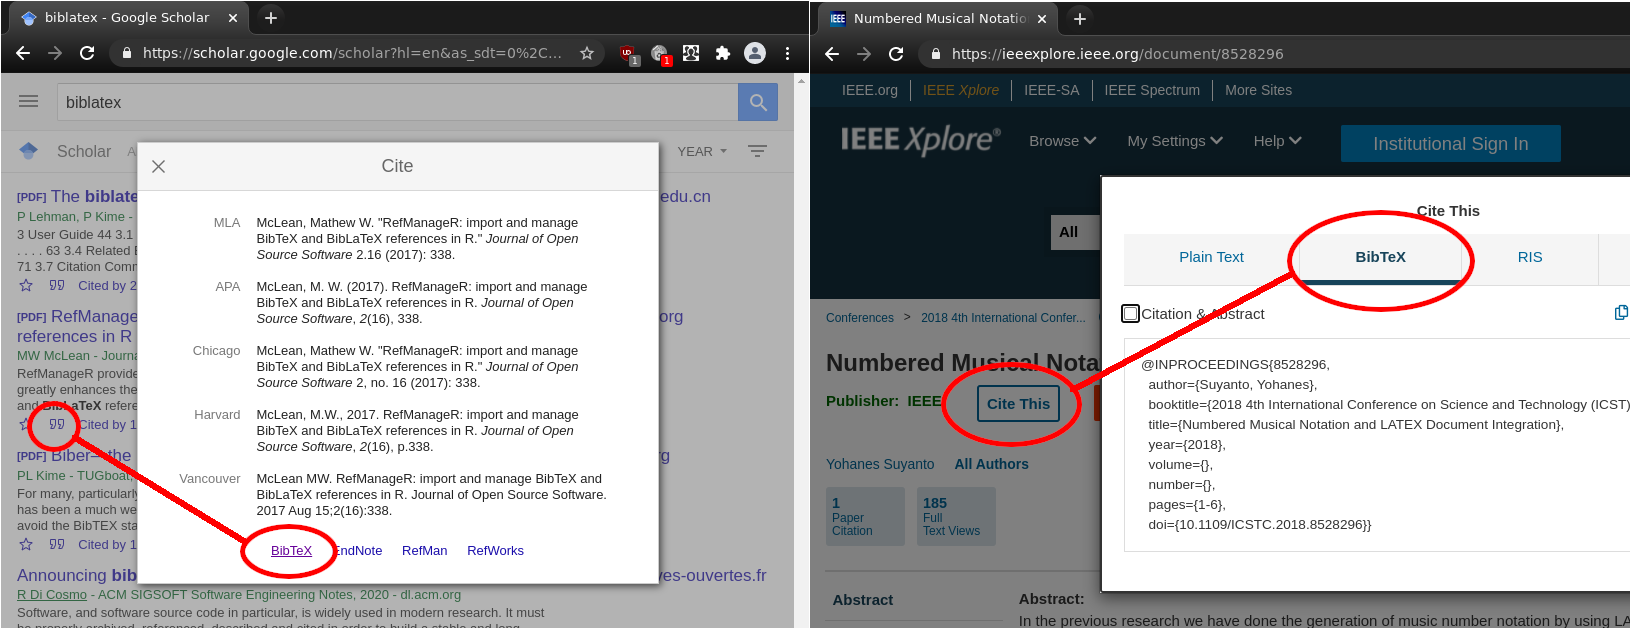
\includegraphics[width=\textwidth]{bibtex_gscholar_ieeexplore}}
  \caption{BibTeX entries from Google Scholar (left) or IEEE Xplore (right)}
  \label{fig:bibtex}
\end{figure}

Let's also try a long quote from the \citetitle{un:udhr}
\begin{quote}
(1) Everyone has the right to education. Education shall be free, at least in the elementary and fundamental stages. Elementary education shall be compulsory. Technical and professional education shall be made generally available and higher education shall be equally accessible to all on the basis of merit.

(2) Education shall be directed to the full development of the human personality and to the strengthening of respect for human rights and fundamental freedoms. It shall promote understanding, tolerance and friendship among all nations, racial or religious groups, and shall further the activities of the United Nations for the maintenance of peace.

(3) Parents have a prior right to choose the kind of education that shall be given to their children. \cite[article 26]{un:udhr}
\end{quote}

%TODO example with cite interview/conversation (unpublished or misc)
%https://tex.stackexchange.com/questions/111363/exclude-fullcite-citation-from-bibliography
\textit{Quisque augue} est, \textbf{elementum ac porttitor} non, porttitor ac orci. Donec hendrerit, ligula ac luctus egestas, sem dolor pretium nunc, sed vehicula magna diam a massa. Donec mattis, arcu et tempor mattis, risus tortor ultrices metus, nec sodales sem dolor eu elit.

Nullam egestas enim at odio pellentesque bibendum.

\subsection{Subsection}
Donec et sapien ac leo condimentum vulputate id et tellus. Maecenas hendrerit malesuada interdum. Aenean dignissim sem faucibus elit congue faucibus id non risus. Morbi at dui non tortor pellentesque consequat non eget urna. Cras in sapien dui, a tincidunt velit.
\reaction{\label{eq:reaktio}$\underset{\text{+II}}{\ce{2Fe^2+}}$ + $\underset{\text{+I\;-I}}{\ce{H2O2}}$ + $\underset{\text{+I\;-II}}{\ce{2H3O^+}}$ <=> $\underset{\text{+III}}{\ce{2Fe^3+}}$ + $\underset{\text{+I\;-II}}{\ce{4H2O}}$}
Työn aluksi rauta(II)ionit hapetetaan rauta(III)ioneiksi väkevällä vetyperoksidilla, kuten reaktion~\ref{eq:reaktio} hapetusluvuista nähdään (rauta hapettuu, happi pelkistyy).
\reaction{Fe^3+( \emph{aq} ) + 3OH^-( \emph{aq} ) + $(x-1)$H2O( \emph{l} ) -> FeOOH $\cdot$ $x$(H2O)( \emph{s} )}
Rauta(III)ionit saostetaan emäksen (\ce{NH3}) avulla ja saadaan tuotteeksi kidevedellinen rauta(III)hydroksidi. Saatu saostuma pestään \ce{NH4NO3}:lla.
\reaction{FeOOH $\cdot$ $x$(H2O)( \emph{s} ) ->T[$\Delta$900-1000\celsius] Fe2O3( \emph{s} )}

\subsection{Subsection with \texorpdfstring{\Gls{maths}}{Mathematics}}%gls inside chapter/section/... will generate hyperref warning (link inside link in table of content), to avoid that, use the \texorpdfstring
Donec et sapien ac leo condimentum vulputate id et tellus. Maecenas hendrerit malesuada interdum. Aenean dignissim sem faucibus elit congue faucibus id non risus. Morbi at dui non tortor pellentesque consequat non eget urna. Cras in sapien dui, a tincidunt velit. Tertiäärinen butyylikloridi reagoi veden kanssa oheisen reaktion mukaisesti:
\reaction{(CH3)3CCl + 2H2O -> (CH3)3COH+H3O+ +Cl-}
Kyseessä on ensimmäisen kertaluvun reaktio, joten reaktion nopeus on
\begin{align}
v=-\frac{\mathrm{d}[\tn{t-ButCl}]}{\mathrm{d}t}=\frac{\mathrm{d}[\tn{HCl}]}{\mathrm{d}t}=k[\tn{t-ButCl}]
\end{align}
Jos tarkastellaan lähtöaineen t-butyylikloridin häviämistä saadaan
\begin{align}
\frac{\mathrm{d}[\tn{t-ButCl}]}{[\tn{t-ButCl}]}&=-k\mathrm{d}t \\
\int \frac{\mathrm{d}[\tn{t-ButCl}]}{[\tn{t-ButCl}]}&=-k \int \mathrm{d}t \\
\ln \int_{[\tn{t-ButCl}]_0}^{[\tn{t-ButCl}]} [\tn{t-ButCl}]&=-k\int_0^t t \\
\ln \left( \frac{[\tn{t-ButCl}]}{[\tn{t-ButCl}]_0} \right)&=-kt
\end{align}
Ionivahvuus lasketaan kaavalla.
\begin{align}
I&=\frac{1}{2}\cdot\sum z_i^2c_i \\
z_i&= \tn{ionin varausluku} \nonumber \\
c_i&= \tn{ionin konsentraatio} \nonumber
\end{align}
Aktiivisuuskerroin $\gamma_\pm$ lasketaan kaavalla.
\begin{align}
\log \gamma_\pm &= -\left|z_+\cdot z_-\right|A\cdot I^{\frac{1}{2}} \\
A &= \tn{0,509 (lämpötilassa 25\celsius}) \nonumber \\
I &= \tn{ionivahvuus} \nonumber \\
z &= \tn{ionien varaus} \nonumber
\end{align}

\section{Section with Source Code}
Donec et sapien ac leo condimentum vulputate id et tellus. Maecenas hendrerit malesuada interdum. Aenean dignissim sem faucibus elit congue faucibus id non risus. Morbi at dui non tortor pellentesque consequat non eget urna. Cras in sapien dui, a tincidunt velit.

%For sharelatex users, use space instead of tab to avoid ^^I
\begin{code}
  \begin{minted}{php}
<?php
$username = $_POST["username"];
//maybe not?
if ($userName){
  ?>
  <h2>Hello <?= $username ?>!</h2>
  <p>your message got received.</p>
  <?php
}
?>
\end{minted}
\captionof{listing}{Descriptive Caption Text (e.g. this \gls{php} code do blah)}
  \label{code:testphp}
\end{code}


As see in listing \ref{code:testphp}, blah. It is also possible to have code inline, for example \mintinline{sql}{SELECT * FROM user WHERE age >= 18} that was \gls{sql}.
The lisings \ref{code:htmlfull} and \ref{code:htmlpart} show how to load code from an external source file. In the case of listing \ref{code:htmlpart} it only take few line out of the source code file.

\begin{code}
  \inputminted{html}{code/html5_sample.html}
  \captionof{listing}{Some \gls{html} code}
  \label{code:htmlfull}
\end{code}
 Donec et sapien ac leo condimentum vulputate id et tellus. Maecenas hendrerit malesuada interdum. Aenean dignissim sem faucibus elit congue faucibus id non risus.

 \begin{code}
   \inputminted[firstline=3,lastline=6]{html}{code/html5_sample.html}
   \captionof{listing}{The \mintinline{html}{<head>} section of an \gls{html} page}
  \label{code:htmlpart}
\end{code}


 Morbi at dui non tortor pellentesque consequat non eget urna. Cras in sapien dui, a tincidunt velit.


\section{Section with Table}
Donec et sapien ac leo condimentum vulputate id et tellus. Maecenas hendrerit malesuada interdum. Aenean dignissim sem faucibus elit congue faucibus id non risus. Morbi at dui non tortor pellentesque consequat non eget urna. Cras in sapien dui, a tincidunt velit.

\begin{table}[h]
  \centering
  \caption{Some data}%IMPORTANT the caption must be before the tabular, so it will be on top of the table (there are other tricks to force it on top; but this one is straightforward).
  \vspace{-16.5pt}%time to time, spacing between caption and table can go too big...
  \begin{tabular}{| l | >{\centering\arraybackslash}p{.5\textwidth} |}
    \hline
    Test 1 & test 1234 test \\
    \hline
    Some more data comes here & with more values and if the text is very long it will disappear out of the box unless you force the column size :( You can use e.g. \textbackslash raggedright or \textbackslash centering (as in this example) to avoid hyphenization of long words\ldots \\
    \hline
  \end{tabular}
  \label{table:some_data}
\end{table}

As presented in table \ref{table:some_data}: Donec et sapien ac leo condimentum vulputate id et tellus. Maecenas hendrerit malesuada interdum. Aenean dignissim sem faucibus elit congue faucibus id non risus. Morbi at dui non tortor pellentesque consequat non eget urna. Cras in sapien dui, a tincidunt velit.

\begin{table}[h]
  \centering
  \caption{Another table with tabularx}
  \begin{tabularx}{.95\textwidth}{| l | >{\centering\arraybackslash} X |}
    \hline
    Test 1 & test 1234 test \\
    \hline
    Some more data comes here & with more values and if the text is very long it will disappear out of the box unless you force the table size :( \\
    \hline
  \end{tabularx}
  \label{table:some_data2}
\end{table}

As presented in table \ref{table:some_data2}: Donec et sapien ac leo condimentum vulputate id et tellus. Maecenas hendrerit malesuada interdum. Aenean dignissim sem faucibus elit congue faucibus id non risus. Morbi at dui non tortor pellentesque consequat non eget urna. Cras in sapien dui, a tincidunt velit.

Donec et sapien ac leo condimentum vulputate id et tellus. Maecenas hendrerit malesuada interdum. Aenean dignissim sem faucibus elit congue faucibus id non risus. Morbi at dui non tortor pellentesque consequat non eget urna. Cras in sapien dui, a tincidunt velit.

\begin{table}[htbp]
  \centering
  \caption{Booktabs example}
  \vspace{-16.5pt}
    \begin{tabular}{rrrr}
    \toprule
    t (s) & [HCl] & [t-ButCl] & $\ln\frac{[t-ButCl]}{[t-ButCl]_0}$ \\
    \midrule
    0     & 4,02  & 160,88 & 0,00 \\
    10    & 63    & 101,9 & -0,46 \\
    20    & 115,2 & 49,7  & -1,17 \\
    30    & 141,3 & 23,6  & -1,92 \\
    40    & 157,9 & 7     & -3,13 \\
    50    & 161   & 3,9   & -3,72 \\
    60    & 164,3 & 0,6   & -5,59 \\
    70    & 163,5 & 1,4   & -4,74 \\
    80    & 163,8 & 1,1   & -4,99 \\
    90    & 164,1 & 0,8   & -5,30 \\
    100   & 164,3 & 0,6   & -5,59 \\
    \bottomrule
    \end{tabular}
  \label{tab:thisislabel}
\end{table}

As presented in table \ref{tab:thisislabel}: Donec et sapien ac leo condimentum vulputate id et tellus. Maecenas hendrerit malesuada interdum. Aenean dignissim sem faucibus elit congue faucibus id non risus. Morbi at dui non tortor pellentesque consequat non eget urna. Cras in sapien dui, a tincidunt velit.

%Dummy content to use some space...
\vspace{21.5pt}
\chapter{Dummy Content}

Lorem ipsum dolor sit amet, consectetur adipiscing elit. Aliquam aliquam aliquam purus, in ornare nulla imperdiet molestie. Nam tempus erat eu dui rhoncus et vestibulum mi elementum. Ut porttitor elit sit amet justo dignissim sit amet sagittis massa egestas. Mauris sed dolor eget dui fermentum sodales ut eu nibh. 

Quisque augue est, elementum ac porttitor non, porttitor ac orci. Donec hendrerit, ligula ac luctus egestas, sem dolor pretium nunc, sed vehicula magna diam a massa. Donec mattis, arcu et tempor mattis, risus tortor ultrices metus, nec sodales sem dolor eu elit. Nullam egestas enim at odio pellentesque bibendum. 

Donec et sapien ac leo condimentum vulputate id et tellus. Maecenas hendrerit malesuada interdum. Aenean dignissim sem faucibus elit congue faucibus id non risus. Morbi at dui non tortor pellentesque consequat non eget urna. Cras in sapien dui, a tincidunt velit.

% Sample content to demonstrate tikzpicture
\vspace{21.5pt}
\chapter{Graph}

Data to plot the graph \ref{fig:stdplot} are in data.dat file.
Lorem ipsum dolor sit amet, consectetur adipiscing elit. Aliquam aliquam aliquam purus, in ornare nulla imperdiet molestie. Nam tempus erat eu dui rhoncus et vestibulum mi elementum. Ut porttitor elit sit amet justo dignissim sit amet sagittis massa egestas. Mauris sed dolor eget dui fermentum sodales ut eu nibh.
\begin{figure}[htbp]
  \centering
    \begin{tikzpicture}
        \pgfplotsset{width=12cm, legend style={font=\footnotesize}}
    \begin{axis}[
    xlabel={c (mg/l)},
    ylabel={A},
    legend pos=north west,
    ymajorgrids=true,
    grid style=dashed
]

\addplot [only marks, blue] table {data.dat};
\addplot [no markers, thick, red] table[
x=c,
y={create col/linear regression}] {data.dat};
\addlegendentry{data}
\addlegendentry{%
$\pgfmathprintnumber{\pgfplotstableregressiona}x
\pgfmathprintnumber[print sign]{\pgfplotstableregressionb}$}
\end{axis}
\end{tikzpicture}
\caption{Simple linear regression plot (cannot get $r^2$ value)}
\label{fig:stdplot}
\end{figure}

Quisque augue est, as seen in figure \ref{fig:stdplot} elementum ac porttitor non, porttitor ac orci. Donec hendrerit, ligula ac luctus egestas, sem dolor pretium nunc, sed vehicula magna diam a massa. Donec mattis, arcu et tempor mattis, risus tortor ultrices metus, nec sodales sem dolor eu elit. Nullam egestas enim at odio pellentesque bibendum.

Donec et sapien ac leo condimentum vulputate id et tellus. Maecenas hendrerit malesuada interdum. Aenean dignissim sem faucibus elit congue faucibus id non risus. Morbi at dui non tortor pellentesque consequat non eget urna. Cras in sapien dui, a tincidunt velit.

\section{Section}

Lorem ipsum dolor sit amet, consectetur adipiscing elit. Aliquam aliquam aliquam purus, in ornare nulla imperdiet molestie. Nam tempus erat eu dui rhoncus et vestibulum mi elementum.
\tikzstyle{palikka} = [rectangle, rounded corners, minimum width=1cm, minimum height=1cm, text centered, text width=2cm, draw=black, fill=red!30]
\tikzstyle{arrow} = [thick,->,>=stealth]
\begin{figure}[htbp]
\centering
\begin{tikzpicture}[node distance=2.75cm]
\node[label=90:Label] (yksi) [palikka] {Lorem};
\node (kaksi) [palikka, right of=yksi] {ipsum};
\node (kolme) [palikka, below of=kaksi,  yshift=1cm] {dolor};
\node (neljä) [palikka, left of=kolme] {sit};
\node (viisi) [palikka, below of=neljä, yshift=1cm] {amet};
\draw [arrow] (yksi) -- (kaksi);
\draw [arrow] (kaksi) -- node[anchor=west] {tekstiä} (kolme);
\draw [arrow] (kolme) -- (neljä);
\draw [arrow] (neljä) -- (viisi);
\end{tikzpicture}
\caption{Example tikz-picture}
\label{fig:tikz}
\end{figure}

As seen in figure \ref{fig:tikz}, ut porttitor elit sit amet justo dignissim sit amet sagittis massa egestas. Mauris sed dolor eget dui fermentum sodales ut eu nibh.

\section{Section}

Lorem ipsum dolor sit amet, consectetur adipiscing elit. Aliquam aliquam aliquam purus, in ornare nulla imperdiet molestie. Nam tempus erat eu dui rhoncus et vestibulum mi elementum. Ut porttitor elit sit amet justo dignissim sit amet sagittis massa egestas. Mauris sed dolor eget dui fermentum sodales ut eu nibh.


%----------------------------------------------------------------------------------------
%	BIBLIOGRAPHY REFERENCES
%----------------------------------------------------------------------------------------

% Bibliography.
% Normally you do not edit this file.
% To add bibliography in your text, add them first in the biblio.bib file and
% reference them with the \cite{} command in your text. Check also \citeauthor
% and \citeyear (e.g. for copied figure caption), the \cites for multi-cites
% with page numbers,...

\clearpage
%line space
%\singlespacing %removed otherwise the appendix are also single space
\begin{singlespacing}
\vspace*{-16pt}
\printbibliography[title=\IfLanguageName{finnish}{Lähteet}{References}]
\end{singlespacing}

%for conting the pages
\label{LastPage}~


%----------------------------------------------------------------------------------------
%	APPENDICES
%----------------------------------------------------------------------------------------

% Appendix
% Normally, you do not have to edit this file.

%start appendix
\appendix
%no page number for appendix in table of content
\addtocontents{toc}{\cftpagenumbersoff{chapter}}
%appendix sections and subsections not in table of content
\settocdepth{chapter}
%add "Appendices" in the table of content
\addappheadtotoc
%have Appendix 1 (instead of Appendix A)
\renewcommand{\thechapter}{\arabic{chapter}}

\newcommand\liite[1]{
%each appendix start on a new page
\clearpage
%each appendix restart page num to one
\setcounter{page}{1}
%special counter for appendix TODO: this is a ugly quick hack :( Should find a better way to count the page per appendix.
\newtotcounter{appx#1}
%overwrite the header
\makeevenhead{plain}{}{}{\appname \thechapter \\ \thepage\,(\stepcounter{appx#1}\total{appx#1})}
\makeoddhead{plain}{}{}{\appname \thechapter \\ \thepage\,(\stepcounter{appx#1}\total{appx#1})}}



%force smaller vertical spacing in table of content
%!!! There can be some fun depending if the appendices have (sub)sections or not :D
% You will have to play with these numbers and eventually add the \vspace line  before
% some \chapter and force another number.
% To add more fun, time to time the table of content get wrong after a build :(
\addtocontents{toc}{\vspace{11pt}}
\pretocmd{\chapter}{\addtocontents{toc}{\protect\vspace{-24pt}}}{}{}

\liite{1}% This is a hack to have right page numbering for each appendix. Make sure to
% use a unique number for each appendix.
% Appendix
% And demonstrate text references and bibliography references in appendix

\chapter{Some Appendix}\label{appx:first}

Note that every appendix will be a chapter.

Sorry for the ugly hack on how to count the total pages per appendix.


Of course with section and subsection.

\section{Appendix Section}

And you can cite \cite{tobias:book} stuff, it will go into the main bibliography.

Lorem ipsum dolor sit amet, consectetur adipiscing elit. Aliquam aliquam aliquam purus, in ornare nulla imperdiet molestie. Nam tempus erat eu dui rhoncus et vestibulum mi elementum. Ut porttitor elit sit amet justo dignissim sit amet sagittis massa egestas. Mauris sed dolor eget dui fermentum sodales ut eu nibh.

Quisque augue est, elementum ac porttitor non, porttitor ac orci. Donec hendrerit, ligula ac luctus egestas, sem dolor pretium nunc, sed vehicula magna diam a massa. Donec mattis, arcu et tempor mattis, risus tortor ultrices metus, nec sodales sem dolor eu elit. Nullam egestas enim at odio pellentesque bibendum.

\subsection{With a Subsection}

Lorem ipsum dolor sit amet, consectetur adipiscing elit. Aliquam aliquam aliquam purus, in ornare nulla imperdiet molestie. Nam tempus erat eu dui rhoncus et vestibulum mi elementum. Ut porttitor elit sit amet justo dignissim sit amet sagittis massa egestas. Mauris sed dolor eget dui fermentum sodales ut eu nibh.

Quisque augue est, elementum ac porttitor non, porttitor ac orci. Donec hendrerit, ligula ac luctus egestas, sem dolor pretium nunc, sed vehicula magna diam a massa. Donec mattis, arcu et tempor mattis, risus tortor ultrices metus, nec sodales sem dolor eu elit. Nullam egestas enim at odio pellentesque bibendum.

Donec et sapien ac leo condimentum vulputate id et tellus. Maecenas hendrerit malesuada interdum. Aenean dignissim sem faucibus elit congue faucibus id non risus. Morbi at dui non tortor pellentesque consequat non eget urna. Cras in sapien dui, a tincidunt velit.
% Sample content to demonstrate appendix in LaTeX. You
% are safe to delete this lines (and the next samples) once you refreshed your LaTeX
% skills (and safe to delete the sample folder and all its file too).

%\addtocontents{toc}{\vspace{11pt}}%fix vertical space for Table of Content
\liite{2}
% Appendix
% Just to have more appendices and more content

\chapter{Dummy Appendix}\label{appx:second}

Lorem ipsum dolor sit amet, consectetur adipiscing elit. Aliquam aliquam aliquam purus, in ornare nulla imperdiet molestie. Nam tempus erat eu dui rhoncus et vestibulum mi elementum. Ut porttitor elit sit amet justo dignissim sit amet sagittis massa egestas. Mauris sed dolor eget dui fermentum sodales ut eu nibh.

Quisque augue est, elementum ac porttitor non, porttitor ac orci. Donec hendrerit, ligula ac luctus egestas, sem dolor pretium nunc, sed vehicula magna diam a massa. Donec mattis, arcu et tempor mattis, risus tortor ultrices metus, nec sodales sem dolor eu elit. Nullam egestas enim at odio pellentesque bibendum.

Donec et sapien ac leo condimentum vulputate id et tellus. Maecenas hendrerit malesuada interdum. Aenean dignissim sem faucibus elit congue faucibus id non risus. Morbi at dui non tortor pellentesque consequat non eget urna. Cras in sapien dui, a tincidunt velit.

Lorem ipsum dolor sit amet, consectetur adipiscing elit. Aliquam aliquam aliquam purus, in ornare nulla imperdiet molestie. Nam tempus erat eu dui rhoncus et vestibulum mi elementum. Ut porttitor elit sit amet justo dignissim sit amet sagittis massa egestas. Mauris sed dolor eget dui fermentum sodales ut eu nibh.

Quisque augue est, elementum ac porttitor non, porttitor ac orci. Donec hendrerit, ligula ac luctus egestas, sem dolor pretium nunc, sed vehicula magna diam a massa. Donec mattis, arcu et tempor mattis, risus tortor ultrices metus, nec sodales sem dolor eu elit. Nullam egestas enim at odio pellentesque bibendum.

Donec et sapien ac leo condimentum vulputate id et tellus. Maecenas hendrerit malesuada interdum. Aenean dignissim sem faucibus elit congue faucibus id non risus. Morbi at dui non tortor pellentesque consequat non eget urna. Cras in sapien dui, a tincidunt velit.

Lorem ipsum dolor sit amet, consectetur adipiscing elit. Aliquam aliquam aliquam purus, in ornare nulla imperdiet molestie. Nam tempus erat eu dui rhoncus et vestibulum mi elementum. Ut porttitor elit sit amet justo dignissim sit amet sagittis massa egestas. Mauris sed dolor eget dui fermentum sodales ut eu nibh.

Quisque augue est, elementum ac porttitor non, porttitor ac orci. Donec hendrerit, ligula ac luctus egestas, sem dolor pretium nunc, sed vehicula magna diam a massa. Donec mattis, arcu et tempor mattis, risus tortor ultrices metus, nec sodales sem dolor eu elit. Nullam egestas enim at odio pellentesque bibendum.

Donec et sapien ac leo condimentum vulputate id et tellus. Maecenas hendrerit malesuada interdum. Aenean dignissim sem faucibus elit congue faucibus id non risus. Morbi at dui non tortor pellentesque consequat non eget urna. Cras in sapien dui, a tincidunt velit.

Lorem ipsum dolor sit amet, consectetur adipiscing elit. Aliquam aliquam aliquam purus, in ornare nulla imperdiet molestie. Nam tempus erat eu dui rhoncus et vestibulum mi elementum. Ut porttitor elit sit amet justo dignissim sit amet sagittis massa egestas. Mauris sed dolor eget dui fermentum sodales ut eu nibh.

Quisque augue est, elementum ac porttitor non, porttitor ac orci. Donec hendrerit, ligula ac luctus egestas, sem dolor pretium nunc, sed vehicula magna diam a massa. Donec mattis, arcu et tempor mattis, risus tortor ultrices metus, nec sodales sem dolor eu elit. Nullam egestas enim at odio pellentesque bibendum.

Donec et sapien ac leo condimentum vulputate id et tellus. Maecenas hendrerit malesuada interdum. Aenean dignissim sem faucibus elit congue faucibus id non risus. Morbi at dui non tortor pellentesque consequat non eget urna. Cras in sapien dui, a tincidunt velit.

Lorem ipsum dolor sit amet, consectetur adipiscing elit. Aliquam aliquam aliquam purus, in ornare nulla imperdiet molestie. Nam tempus erat eu dui rhoncus et vestibulum mi elementum. Ut porttitor elit sit amet justo dignissim sit amet sagittis massa egestas. Mauris sed dolor eget dui fermentum sodales ut eu nibh.

Quisque augue est, elementum ac porttitor non, porttitor ac orci. Donec hendrerit, ligula ac luctus egestas, sem dolor pretium nunc, sed vehicula magna diam a massa. Donec mattis, arcu et tempor mattis, risus tortor ultrices metus, nec sodales sem dolor eu elit. Nullam egestas enim at odio pellentesque bibendum.

Donec et sapien ac leo condimentum vulputate id et tellus. Maecenas hendrerit malesuada interdum. Aenean dignissim sem faucibus elit congue faucibus id non risus. Morbi at dui non tortor pellentesque consequat non eget urna. Cras in sapien dui, a tincidunt velit.

Lorem ipsum dolor sit amet, consectetur adipiscing elit. Aliquam aliquam aliquam purus, in ornare nulla imperdiet molestie. Nam tempus erat eu dui rhoncus et vestibulum mi elementum. Ut porttitor elit sit amet justo dignissim sit amet sagittis massa egestas. Mauris sed dolor eget dui fermentum sodales ut eu nibh.

Quisque augue est, elementum ac porttitor non, porttitor ac orci. Donec hendrerit, ligula ac luctus egestas, sem dolor pretium nunc, sed vehicula magna diam a massa. Donec mattis, arcu et tempor mattis, risus tortor ultrices metus, nec sodales sem dolor eu elit. Nullam egestas enim at odio pellentesque bibendum.

Donec et sapien ac leo condimentum vulputate id et tellus. Maecenas hendrerit malesuada interdum. Aenean dignissim sem faucibus elit congue faucibus id non risus. Morbi at dui non tortor pellentesque consequat non eget urna. Cras in sapien dui, a tincidunt velit.


\addtocontents{toc}{\vspace{11pt}}
\liite{3}
% Appendix to demonstrate R integration

\chapter{R examples}

TODO



%----------------------------------------------------------------------------------------
%	THIS IS THE END
%----------------------------------------------------------------------------------------
\end{document}
